\documentclass[12pt,twoside,openany]{book}
\usepackage[utf8]{inputenc}
\usepackage[T1]{fontenc}
\usepackage[english]{babel}

% Paper size A5 (148 x 210 mm)
\usepackage[a5paper, top=25mm, bottom=20mm, inner=20mm, outer=15mm, footskip=10mm]{geometry}

\usepackage{titlesec}
\usepackage{fancyhdr}
\usepackage{setspace} % For line spacing
\usepackage{graphicx}
\graphicspath{ {images/} }
\usepackage{needspace}
\usepackage{microtype}
\usepackage{csquotes}
\usepackage{ebgaramond} % Professional Garamond font
\usepackage[parfill]{parskip} % Spacing between paragraphs
\usepackage{xcolor}
\usepackage{qrcode} % For generating QR codes directly in PDF
\usepackage[export]{adjustbox} % For image borders
\usepackage[framemethod=TikZ]{mdframed} % For elegant frames around text

% Line spacing - generous for 12pt
\setstretch{1.5}

% Font size handled by documentclass options 14pt

% Section styling - elegant Garamond headers
\titleformat{\chapter}[display]
  {\normalfont\LARGE\bfseries\itshape\centering}{\chaptertitlename\ \thechapter}{5pt}{\LARGE}
\titlespacing*{\chapter}{0pt}{20pt}{20pt}

\setlength{\headheight}{16pt}

% Header/Footer - fixing long title issue
\pagestyle{fancy}
\fancyhf{}
\fancyhead[LE,RO]{\small\thepage}
\fancyhead[RE]{\small\itshape\nouppercase{My Friend Jesus Christ}}
\fancyhead[LO]{\small\itshape\nouppercase{\leftmark}}
\renewcommand{\headrulewidth}{0.4pt}

% Fix for long titles in headers: truncate if needed
\renewcommand{\chaptermark}[1]{\markboth{#1}{}}

% Page transitions
\newcommand{\chapterbreak}{\clearpage}

\usepackage{url}
\usepackage{hyperref}
\begin{document}

\frontmatter

% Cover
\begin{titlepage}
    \centering
    \vspace*{2cm}
    {\Huge \textbf{My Friend Jesus Christ} \par}
    \vspace{1cm}
    {\Large A Quantum Guide for the Modern Soul \par}
    \vfill
    {\Large \textit{A Glimpse of Light} \par}
    \vspace*{3cm}
\end{titlepage}

% Copyright Page
\newpage
\thispagestyle{empty}
\vspace*{12cm}
\begin{center}
    \small
    My Friend Jesus Christ \\
    © 2024 A Glimpse of Light \\
    All rights reserved. \\
    Published on Amazon KDP \\
\end{center}

\tableofcontents

\mainmatter

\chapter*{Introduction: Between Particle and Vibration}
\addcontentsline{toc}{chapter}{Introduction: Between Particle and Vibration}
\markboth{Introduction: Between Particle and Vibration}{Introduction: Between Particle and Vibration}
\vspace{1.5cm}
\begin{figure}[h!]
\centering
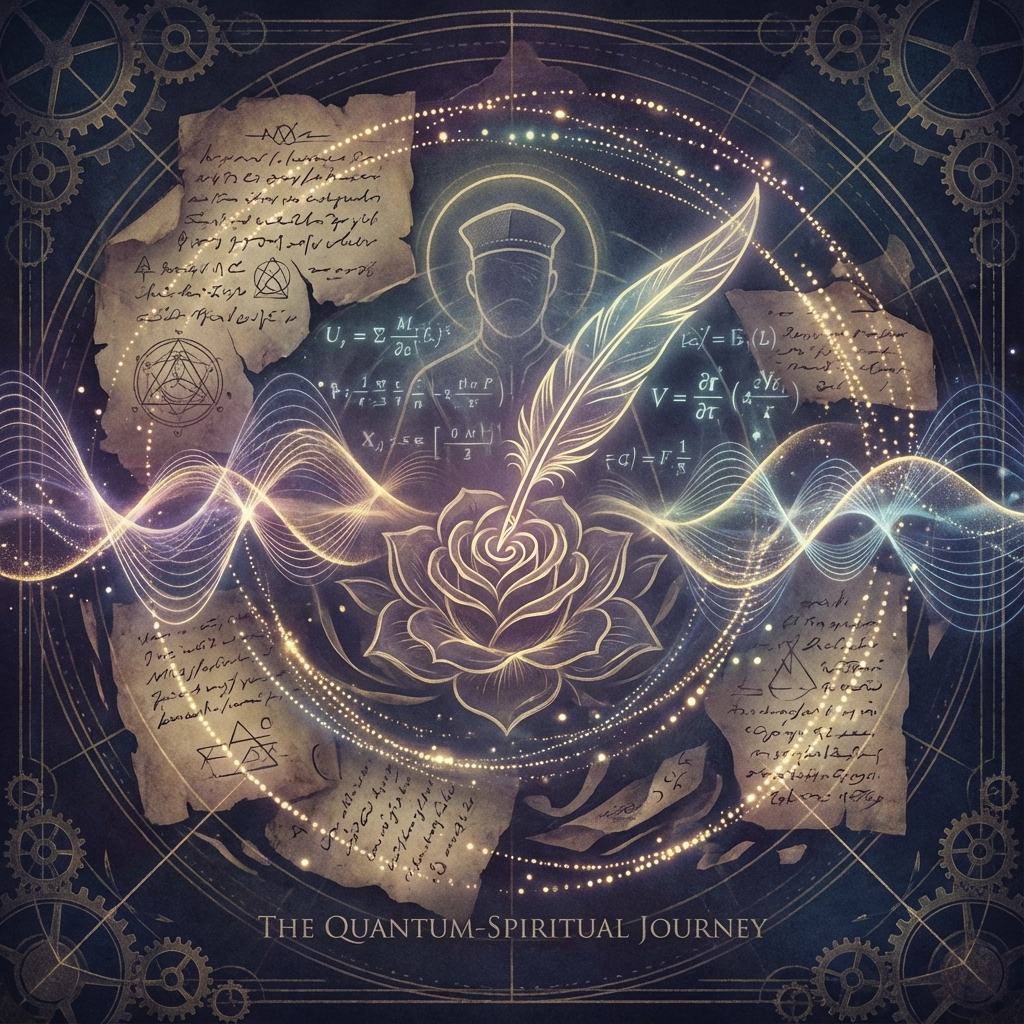
\includegraphics[width=0.85\textwidth,cfbox=gray 0.5pt 3pt]{intro_quantum_luther.png}
\end{figure}

\vspace{1cm}
I. The Soul's Unrest
For as long as I can remember, I have felt a kind of dissonant vibration whenever I approached the great temples of stone. It wasn't a lack of faith; on the contrary, I have always sensed that behind the veil of reality exists an inexhaustible Source of love. My conflict, my silent torment, was born from the contrast between that intuition of an infinite God and the smallness of the boxes into which we tried to fit Him.


I grew up in the heart of Catholicism, breathing the incense and admiring the liturgy, but very soon, that beauty was clouded by an uncomfortable sensation: pride. It pained my soul to hear, implicitly or explicitly, that we had "the truth" and others did not. How could it be that the Creator of a universe of a hundred billion galaxies had a preference for a specific spiritual zip code? I felt we were guilty of a terrible arrogance by not recognizing salvation for other creeds, by looking with pity or superiority at those who sought the light by another path. That exclusivity seemed to me, paradoxically, the most irreligious act of all: limiting God's mercy to our own human borders.


II. The Shadows in the Centers of Power
But my torment went beyond theology. Studying history, I ran into blood-stained walls. The Inquisition, the crusades, the excommunications... I couldn't help thinking: How have we gone from "love your neighbor" to "burn him if he doesn't think like you"?


For years, this pushed me away. I felt rage. I saw the institution and saw only the shadows. However, with time and maturity, I understood something fundamental: the Church, like any human structure, is composed of people. And people are antennas. When fear settles in the centers of power, when the need for control exceeds the need to serve, the collective vibration descends.


The Inquisition was not the work of God, nor was it even the work of "religion" in the abstract. It was the inevitable consequence of a \textbf{low vibration} installed at the top. The fear of losing power, the fear of the different, hatred disguised as zeal... all those are dense, heavy frequencies. And when that density takes over a hierarchy, the result is suffering. Obviously, it is something that Christ himself, my friend Jesus, would never have allowed. He, who stopped the stones against the adulteress, would never have lit a bonfire.


Understanding this allowed me to forgive. I understood that it wasn't "the Church" that failed, but the vibration of the men who, in dark moments, led it. And that, below that dome of power, there were always thousands of priests, nuns, and laypeople vibrating high, feeding the hungry, comforting the sad, keeping the light burning despite the darkness of their leaders.


III. The Quantum Physics of the Spirit
My definitive reconciliation came from science. I have always been fascinated by quantum physics, that branch of knowledge that tells us that reality is not as solid as it seems. It teaches us that every subatomic particle is, at the same time, matter and wave. It is something concrete and, at the same time, it is pure vibration, pure possibility.


That's where everything clicked. The Lord's Prayer, the teachings of Jesus... they weren't rigid moral rules, they were quantum physics instructions!


When Jesus tells us "fear not," he is not giving us a psychological order, he is telling us: "Do not lower your frequency." Fear is a slow, dense vibration that contracts reality. Love, peace, security... are fast, expansive vibrations that create light.


I understood that "falling into temptation" is not eating a cake during Lent. It is the temptation to be dragged down by the gravity of low vibrations: hatred, revenge, envy, pride. When you hate, you become dense. You become a heavy "particle," isolated, disconnected from the whole. When you love, you become a "wave," you expand, you connect with the universal quantum field, with the Father.


IV. A Coffee with Luther
On this journey of understanding, I have often imagined having a coffee with Martin Luther in the 16th century. I think we would have been good friends. He saw that same pride that tormented me. He saw how the structure had become so dense, so concerned with selling indulgences and building marble basilicas, that it had forgotten the vibration of the Gospel.


Luther had the courage to say: "Salvation is not in Rome, it is in your faith." And I would add, from my 21st-century perspective: "Salvation does not depend on following the Pope, but on the frequency of your heart."


If your works, if your daily life, are done from the high vibration of love, there is no doubt that you are saved. Because "being saved" is not a ticket to join a VIP club after you die. Being saved is living, here and now, in the frequency of Paradise. It is being in tune with the Source.


If a Buddhist, an atheist, or a Christian vibrates in unconditional love, they are on the same frequency. They are "in God." And no bull, no decree, can change that physical and spiritual reality. Salvation is a matter of resonance, not bureaucracy.


V. The Light that Prevails
That is why I am writing this book. Not to attack religion, but to rescue its vibrational essence. I write from love, having healed that pity I felt for institutional pride. I have stopped looking at the darkness of the Inquisition to look at the light of the mystics, of the anonymous saints, of the good people who, in the name of that same faith, have vibrated so high that they have changed the world.


This book is an invitation to walk with Jesus, not as a severe judge, but as a master of vibration. A friend who teaches us to navigate between Madrid, Las Rozas and Colmenarejo without losing the tune. A guide who reminds us, again and again, that we are light, that we are waves, and that our only duty is to keep the frequency high, no matter what happens around us.


So, dear reader, forget for a moment the dogmas, the guilts, and the inherited fears. Open your mind to the possibility that everything, absolutely everything, is music. And that you have the instrument in your hands to play the most beautiful melody.


Welcome to "My friend Jesus Christ."
\newpage
\chapter{The Encounter in Madrid}
\vspace{1.5cm}
\begin{figure}[h!]
\centering
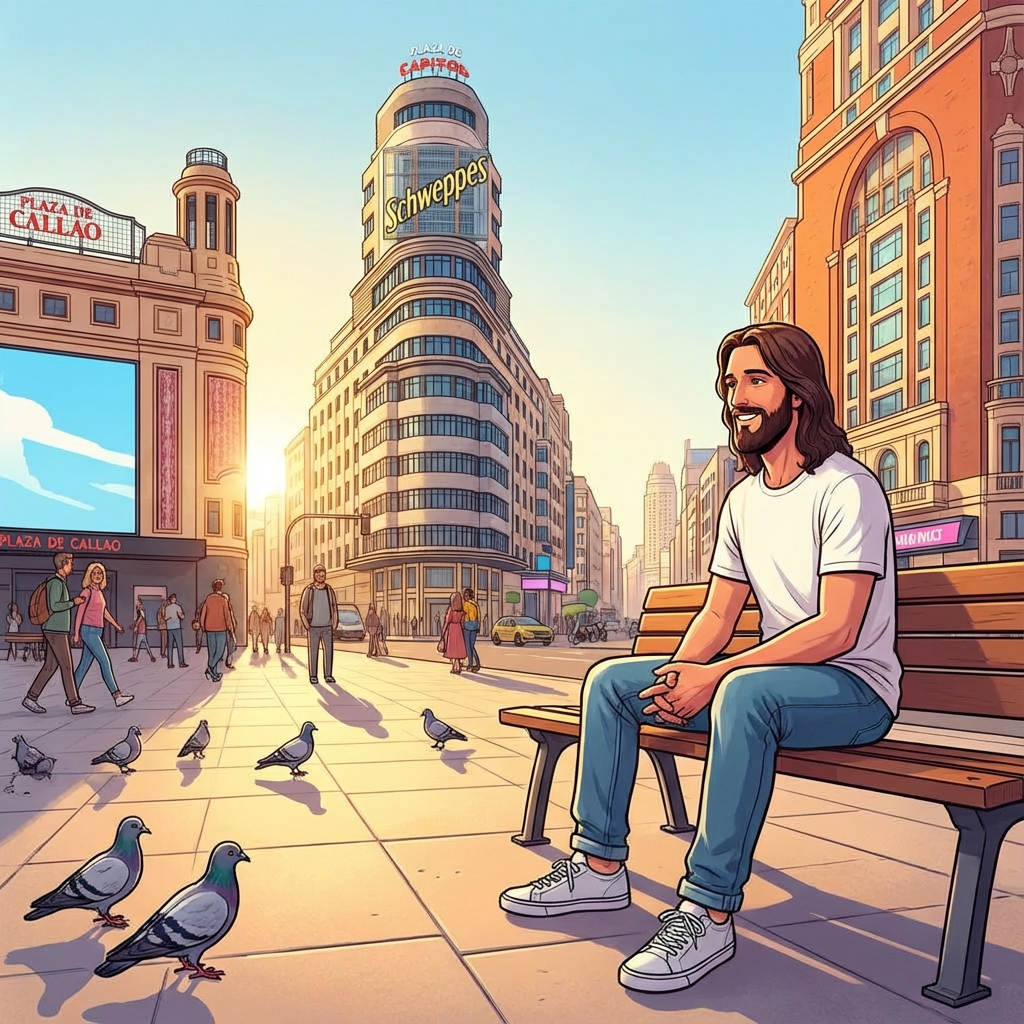
\includegraphics[width=0.85\textwidth,cfbox=gray 0.5pt 3pt]{madrid.png}
\end{figure}

\vspace{1cm}
It was a spring afternoon in Madrid. The sun filtered through the buildings of the Gran Vía, creating games of light and shadow that seemed to dance on the asphalt. I was walking with the usual haste of someone living in the city, with a mind full of noise: emails to answer, bills, worries... vibrating low, very low.


Suddenly, in Callao square, I saw him. He wasn't wearing a tunic, nor sandals, nor did he have a shining halo over his head. He was wearing worn-out jeans, a white t-shirt, and comfortable sneakers. He was sitting on a bench, watching people pass by with a calm smile, a smile that seemed to stop time.


—Hello, Francisco —he said when I passed close by.


I stopped dead in my tracks. No one called me by my full name in the street, and certainly not a stranger. But looking into his eyes, I knew he wasn't a stranger. There was an ancestral familiarity in his gaze, a peace that disarmed any defense.


—Jesus? —I asked, feeling a bit ridiculous.


—The same —he replied, patting the empty space on the bench beside him—. Sit down for a while. You are vibrating at a frequency that is giving me a headache, and I can endure a lot.


I sat down, still stunned.
—Vibrating? —I repeated.


—Yes, vibrating. Everything is vibration, my friend. Fear, haste, anger... are dense, heavy vibrations. They anchor you to the ground and don't let you see the sky, even if you have it right above you.


I looked up. The sky in Madrid was an intense, beautiful blue. I hadn't noticed it until that moment.


—I've come to spend a few days with you —he continued—. Let's go for a walk. You need to remember how to tune the radio of your soul. You are listening to pure static.


And so, in the middle of the bustle of Madrid, began the strangest and most wonderful adventure of my life. Not with miracles of turning water into wine, but with the miracle of transforming my internal noise into music.
\newpage
\chapter{A Walk through Las Rozas}
\vspace{1.5cm}
\begin{figure}[h!]
\centering
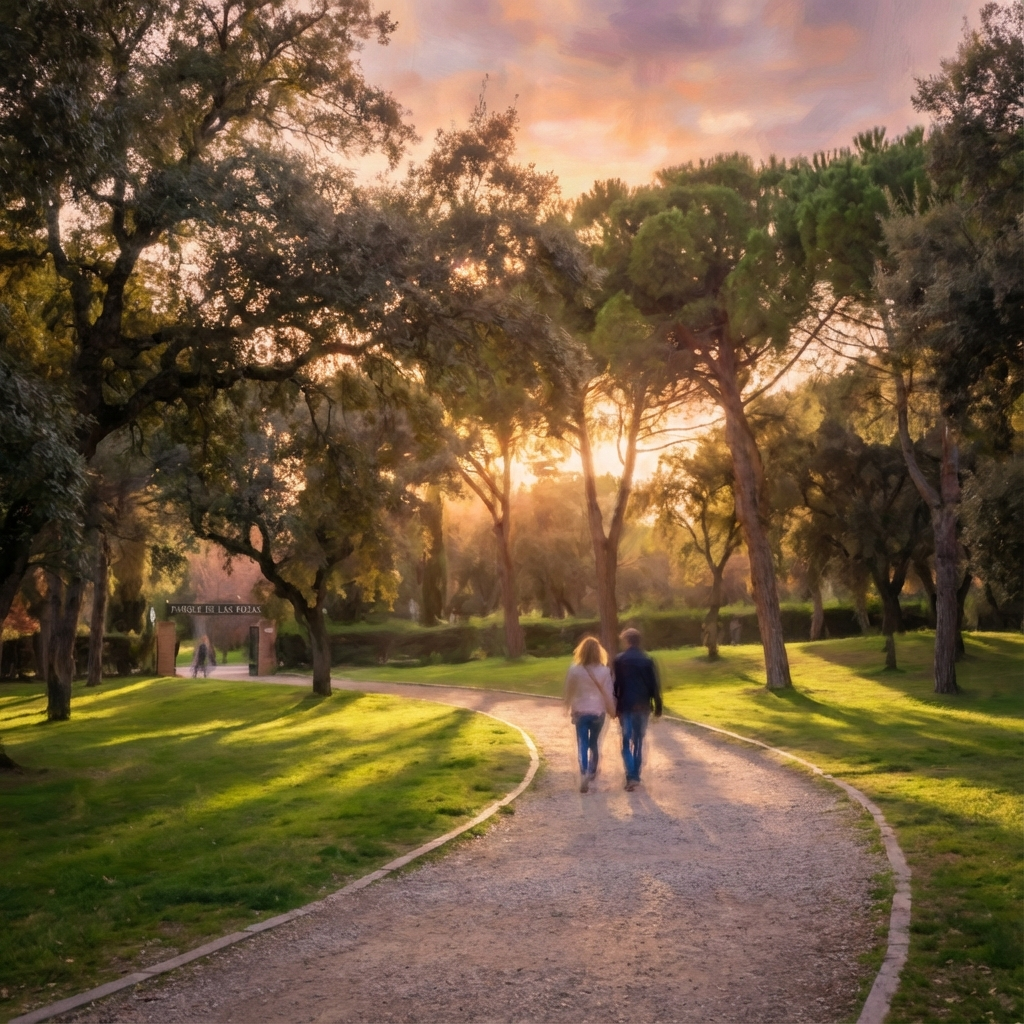
\includegraphics[width=0.85\textwidth,cfbox=gray 0.5pt 3pt]{las_rozas_park.png}
\end{figure}

\vspace{1cm}
The next day, we decided to get away from the center a bit. We went to Las Rozas. Jesus wanted to see how people lived in the outskirts, in those developments where everything seems orderly, but where chaos sometimes hides behind armored doors.


We were walking through Paris Park. He stopped to smell the flowers, to touch the bark of the trees.
—Do you see this? —he told me, pointing to an oak—. He doesn't worry about whether it will rain tomorrow or if it will be sunny. He simply is. He is in his center. He vibrates at the frequency of life.


—It's easy for a tree —I replied—. It doesn't have a mortgage.


Jesus laughed out loud. A clean, infectious laugh.
—The mortgage... the great modern monster. Look, Francisco, the problem isn't the bank debt. The problem is the debt you think you have with the future. You live paying in advance with your anxiety for a time that doesn't yet exist.


We sat on the grass. A dog came running and licked his hand. He petted it tenderly.
—"Give us this day our daily bread" —he whispered—. People think I only talk about food. I'm talking about the energy needed for the \textit{now}. When you worry about next month, you are spending today's energy on an imaginary problem. You lower your vibration. You weaken yourself.


—And how do you raise the vibration? —I asked, feeling that I was beginning to understand.


—By being grateful —he said, looking at the artificial lake—. Gratitude is the elevator of the soul. If you are grateful for this sun, this air, this moment... you go up. If you complain about what you lack... you go down. It's basic spiritual physics.


In Las Rozas, between villas and high-end cars, I learned that true wealth was not in what we possessed, but in the ability to enjoy what was already there, free, for everyone.
\newpage
\chapter{Vibration and Silence}
\vspace{1.5cm}
\begin{figure}[h!]
\centering
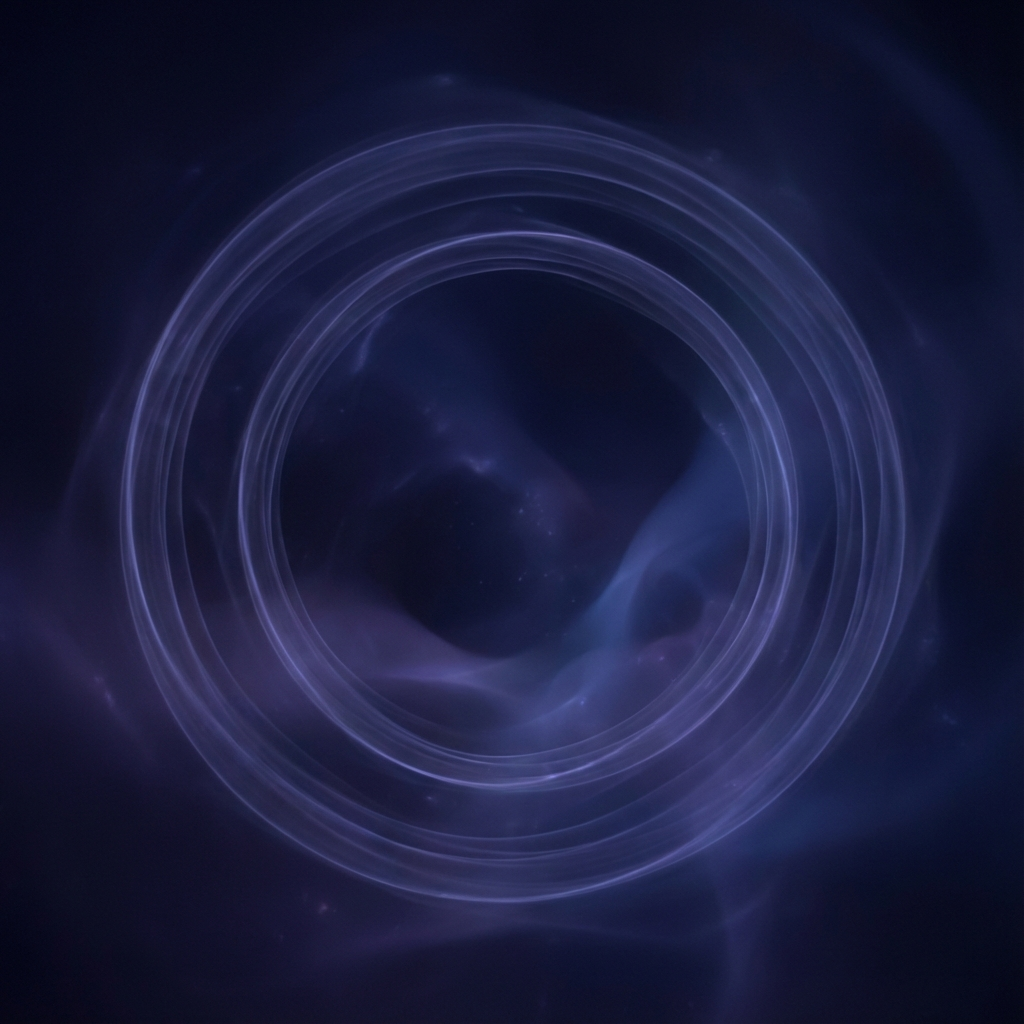
\includegraphics[width=0.85\textwidth,cfbox=gray 0.5pt 3pt]{silence_vibration.png}
\end{figure}

\vspace{1cm}
We took the bus towards the mountains. The landscape was changing, becoming greener, wilder. Jesus looked out the window like a child on his first excursion.


—The noise —he said suddenly—. It is the great disease of this century. Not the noise of cars, but the noise of screens, of notifications, of constant opinions.


We arrived at an intermediate point before Colmenarejo. We got off on a dirt road.
—Let's practice silence —he proposed.


—Stay quiet?


—Not just shut your mouth. Shut your mind. I want you to listen to the vibration of the universe.


We walked in silence for an hour. At first, my mind was a washing machine spinning thoughts: 'What am I doing here walking with Jesus Christ?', 'Have I gone crazy?', 'I have to call my mother...'. But little by little, the rhythm of my steps and the calm breathing of my companion calmed me down.


We stopped at a high point from where the horizon could be seen.
—Close your eyes —he whispered to me—. Feel.


I did it. And for the first time in a long time, I didn't feel fear. I felt a kind of soft, warm hum. As if the air were hugging me.


—That's it —he said, as if he could read my feeling—. That is to vibrate high. It is the frequency of Love. Not the romantic love of the movies, but the Love that holds atoms together. When you are there, nothing can touch you. 'Deliver us from evil' is not asking that evil ones do not exist. It is asking to be at a frequency where evil does not reach you, where it does not resonate with you.


I opened my eyes. The world seemed brighter.
—If you vibrate high, the low frequency doesn't see you —he concluded—. It's as if you were invisible to the darkness.
\newpage
\chapter{Colmenarejo and Nature}
\vspace{1.5cm}
\begin{figure}[h!]
\centering
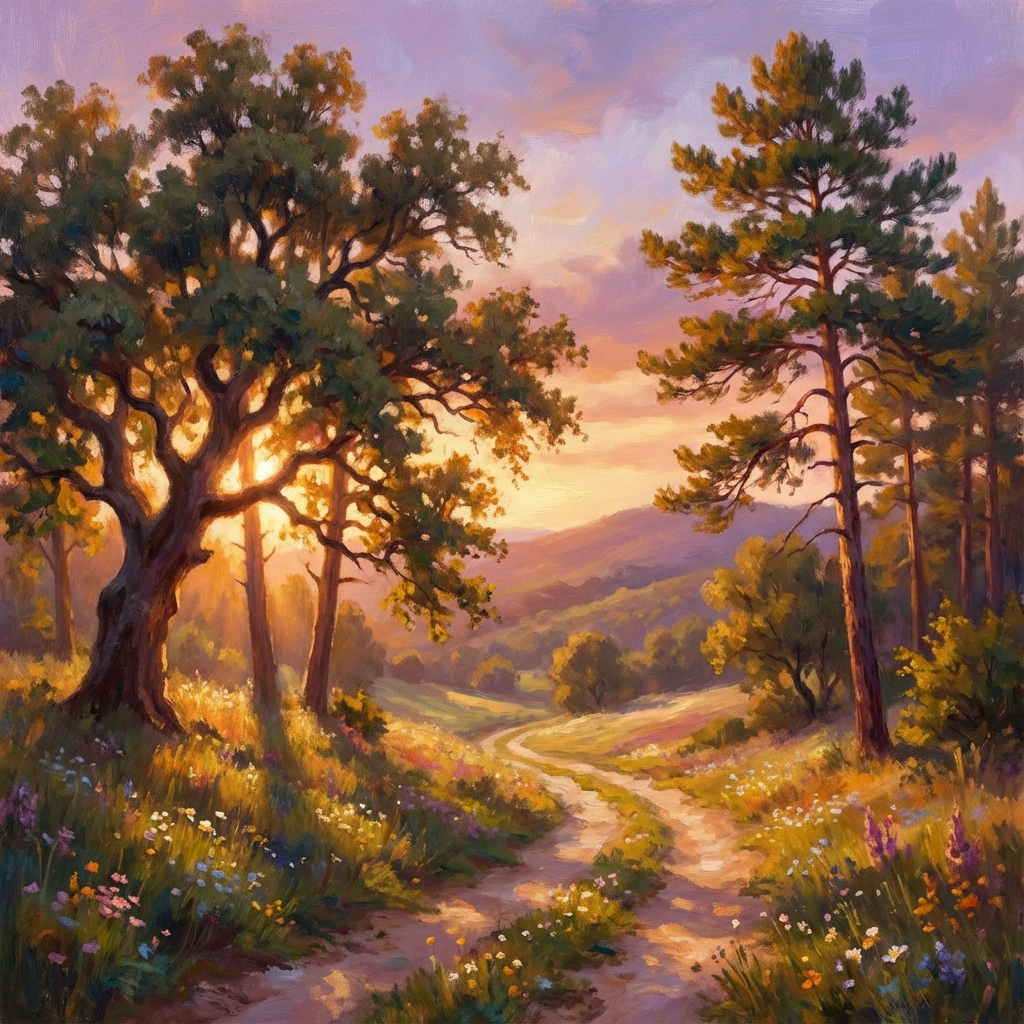
\includegraphics[width=0.85\textwidth,cfbox=gray 0.5pt 3pt]{nature.png}
\end{figure}

\vspace{1cm}
We arrived in Colmenarejo at sunset. The town had that charm of what is halfway between the city and the countryside. We went towards the University area, where there are large open spaces and a different air is breathed.


—It feels better here —Jesus said, breathing deeply—. Nature is the great teacher of vibration. She is never wrong. A pine tree doesn't try to be a holm oak. A river doesn't try to flow upwards.


We sat near the hermitage. The sky was tinged with orange and violet.
—Our Father, who art in heaven... —he began to recite softly—. Do you know where heaven is, Francisco?


—Up there? —I pointed.


He shook his head, smiling.
—Heaven is a state of consciousness. It is that inner place where everything is fine, where there is absolute peace. "Who art in heaven" means that the Source of everything resides in that high vibration. And you have direct access there. You have direct wifi with the Creator, but sometimes you forget the password.


—What is the password?


—Surrender. Stop fighting against what is. Accept. Flow. When you surrender to life, you stop swimming against the current. And then, the current carries you. And the current of life always carries you towards the good, towards the sea.


In Colmenarejo, under the first stars, I understood that praying was not asking for things like someone making a shopping list. Praying was tuning in. It was putting the dial back on the correct frequency to listen to the music that is always playing, even though we are too busy making noise to hear it.
\newpage
\chapter{The Lord's Prayer (Part 1: Father)}
\vspace{1.5cm}
\begin{figure}[h!]
\centering
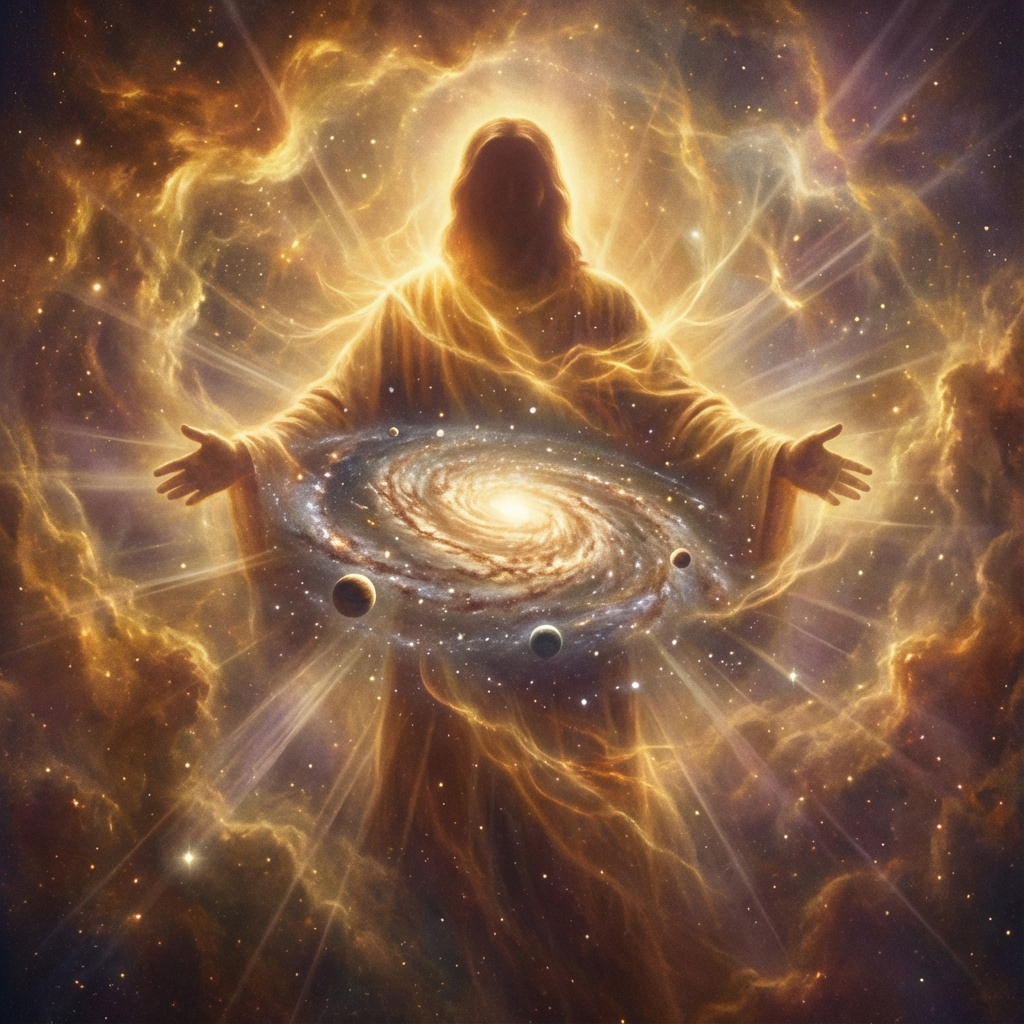
\includegraphics[width=0.85\textwidth,cfbox=gray 0.5pt 3pt]{cosmic_father.png}
\end{figure}

\vspace{1cm}
We returned to Madrid, but this time we went to Retiro. We sat near the Crystal Palace.
—Let's talk about your father —Jesus said suddenly.


I tensed up. My relationship with my father had not always been easy.
—Why?


—Because the prayer starts with "Our Father". And many people get stuck there. If your earthly father was harsh, or absent, or critical, you project that image onto God. You believe that God is a gentleman with a beard who watches you to punish you if you make a mistake.


He picked up a stone from the ground and threw it into the pond. The ripples expanded.
—The word "Father" in Aramaic, \textit{Abwoon}, has a much broader meaning. It is the Source, the Origin, the Breath of Life. It's not a gentleman. It's an Energy. It's the original vibration from which we all come.


—So, he's not a judge?


—Of course not! —he exclaimed—. Does the sun judge the flowers? Does it say to them "you do bloom, I give you light; you do not, you stay in the dark"? The sun shines for all. God is unconditional Love. If you close yourself in a cave, it's not the sun's fault that you're in the dark. It's your choice.


—And why "Our"?


—Because it's not "Mine". It's not the private property of any religion, nor of any person. It belongs to everyone. To the Christian, the Buddhist, the atheist, the tree and the dog. We all come from the same Source. Recognizing that is the first step to vibrate high: Unity. If you see yourself as separate from others, you lower your vibration. If you see yourself as united, you go up.
\newpage
\chapter{The Lord's Prayer (Part 2: Heaven)}
\vspace{1.5cm}
\begin{figure}[h!]
\centering
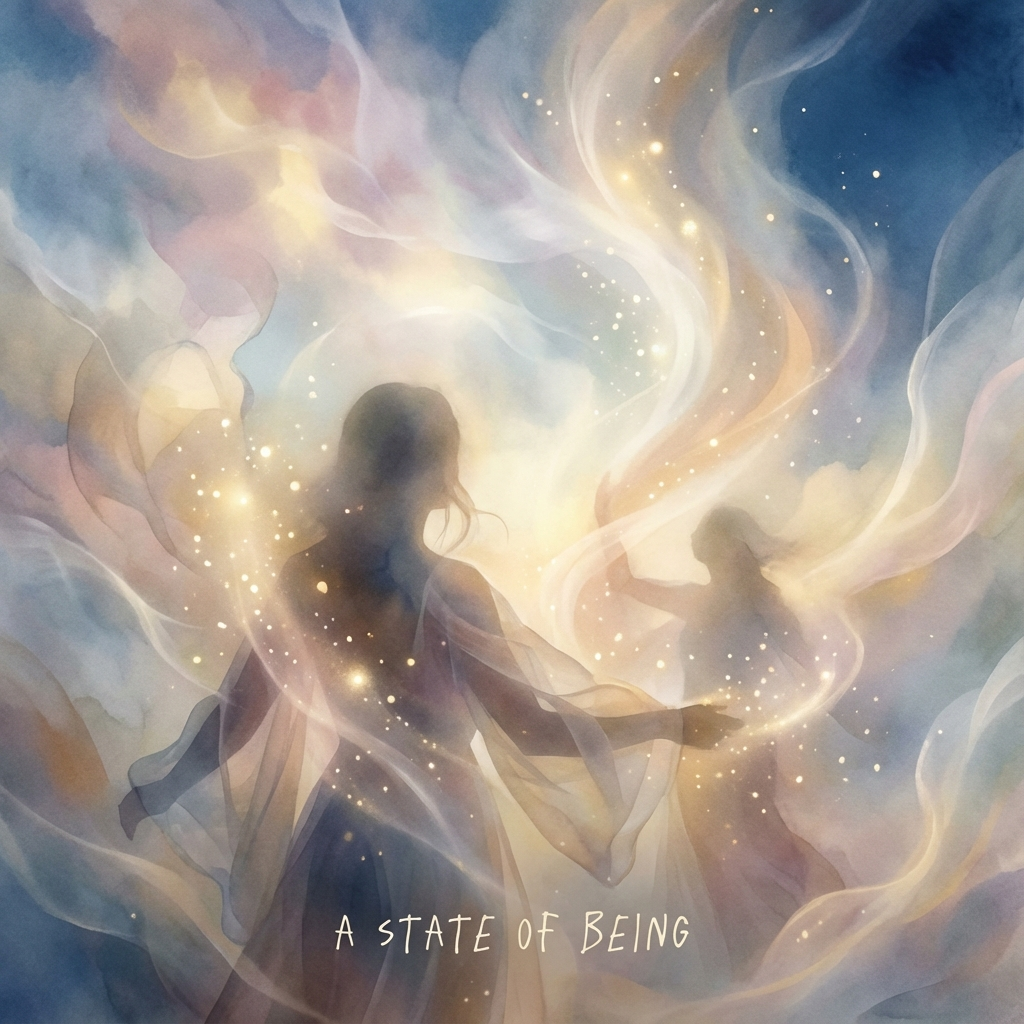
\includegraphics[width=0.85\textwidth,cfbox=gray 0.5pt 3pt]{heaven_state.png}
\end{figure}

\vspace{1cm}
Walking down Gran Vía again, surrounded by glowing advertisements and people with shopping bags, Jesus pointed upwards.
—"Who art in heaven". I already told you in Colmenarejo that heaven is a state of consciousness. But I want you to understand something more.


He stopped in front of a luxury shop window.
—People look for heaven here —he pointed to the expensive watches—. They believe that if they have this, they will be happy. That if they get that job, or that partner, they will touch the sky. But heaven is not a place you go to, it is a place you live from.


—How do you live from heaven here, in the middle of traffic and stress?


—By bringing heaven to earth. That is your mission. "Thy kingdom come". It's not waiting to die to go to a nice place with clouds. It's making this place, here and now, look like that vibration of love and peace.


—That sounds difficult.


—It is if you try to change the world outside without changing the one inside. If you are at peace, if you vibrate in gratitude, you create a small bubble of heaven around you. And if many do that, the bubbles join together. That's how the Kingdom comes. Not with armies, but with calm hearts.


He looked at me fixedly.
—You are a channel. If you are dirty with fear and resentment, the light doesn't pass. If you clean yourself, if you vibrate high, heaven passes through you and reaches the earth. You are a bridge, Francisco. You all are.
\newpage
\chapter{Our Daily Bread}
\vspace{1.5cm}
\begin{figure}[h!]
\centering
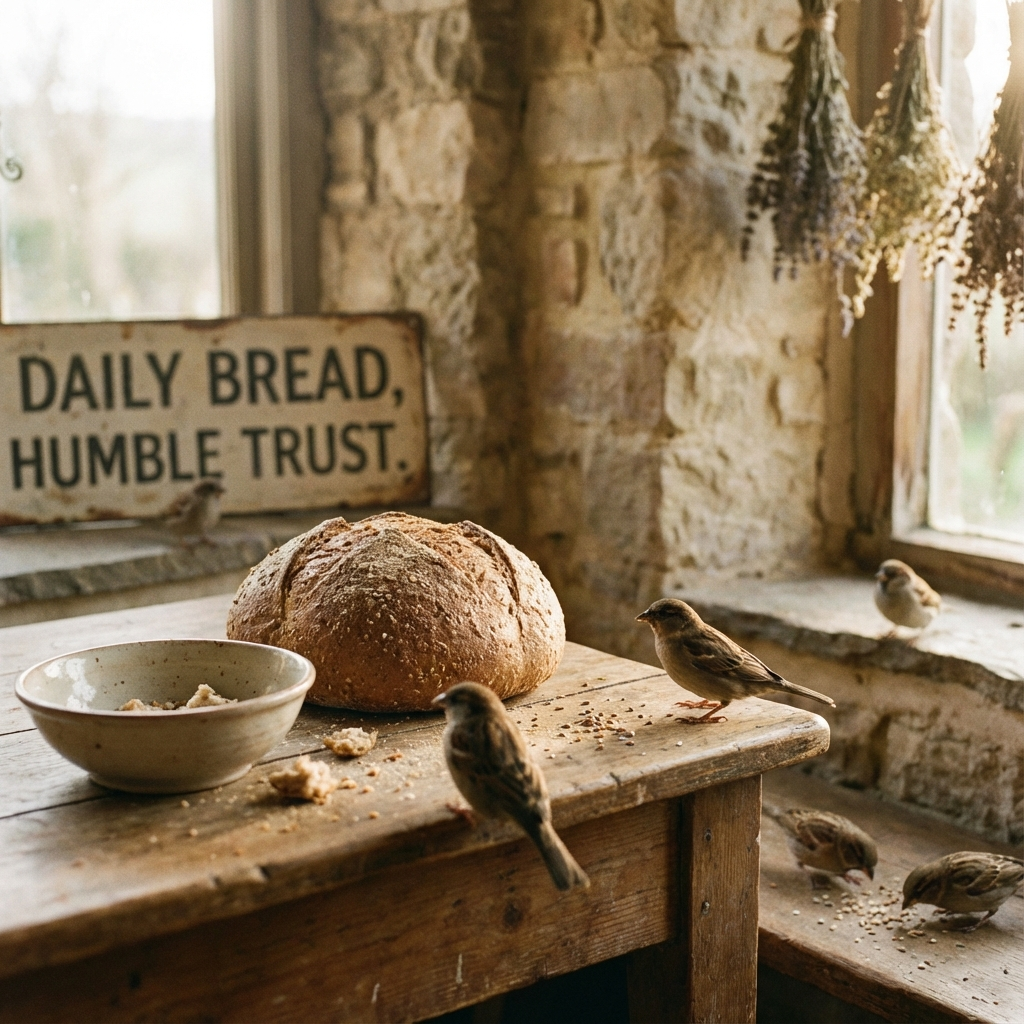
\includegraphics[width=0.85\textwidth,cfbox=gray 0.5pt 3pt]{bread_sparrows.png}
\end{figure}

\vspace{1cm}
We were eating a calamari sandwich in Plaza Mayor. Jesus enjoyed it as if it were the most exquisite delicacy in the world.
—This is sacred —he said with his mouth full.


—The sandwich?


—The act of nourishing oneself. "Give us this day our daily bread".


He wiped himself with a paper napkin.
—People live with fear of scarcity. They accumulate, they store, they fear losing. That is a vibration of lack. When you ask for "today's" bread, you are trusting that tomorrow there will also be some.


—But one must be far-sighted...


—Being far-sighted is fine. Living distressed by the future is a lack of faith in Life. Look at the sparrows —he pointed to some birds pecking at crumbs—. They don't have granaries, and yet, they eat. Life sustains Life.


—And what about the people who have nothing to eat?


His face darkened a bit.
—That is not because bread is lacking. It is because selfishness is overflowing. If everyone vibrated in generosity, if everyone understood that we are one, no one would go hungry. The problem is distribution, not provision. The Universe is abundant. The human mind is what creates scarcity.


He took the last bite.
—The "bread" is also information, knowledge, love. Everything that nourishes you. Ask for what you need for today, to be your best version today. Do not ask to accumulate and feel secure. The only real security is your connection to the Source.
\newpage
\chapter{Forgiveness and Debts}
\vspace{1.5cm}
\begin{figure}[h!]
\centering
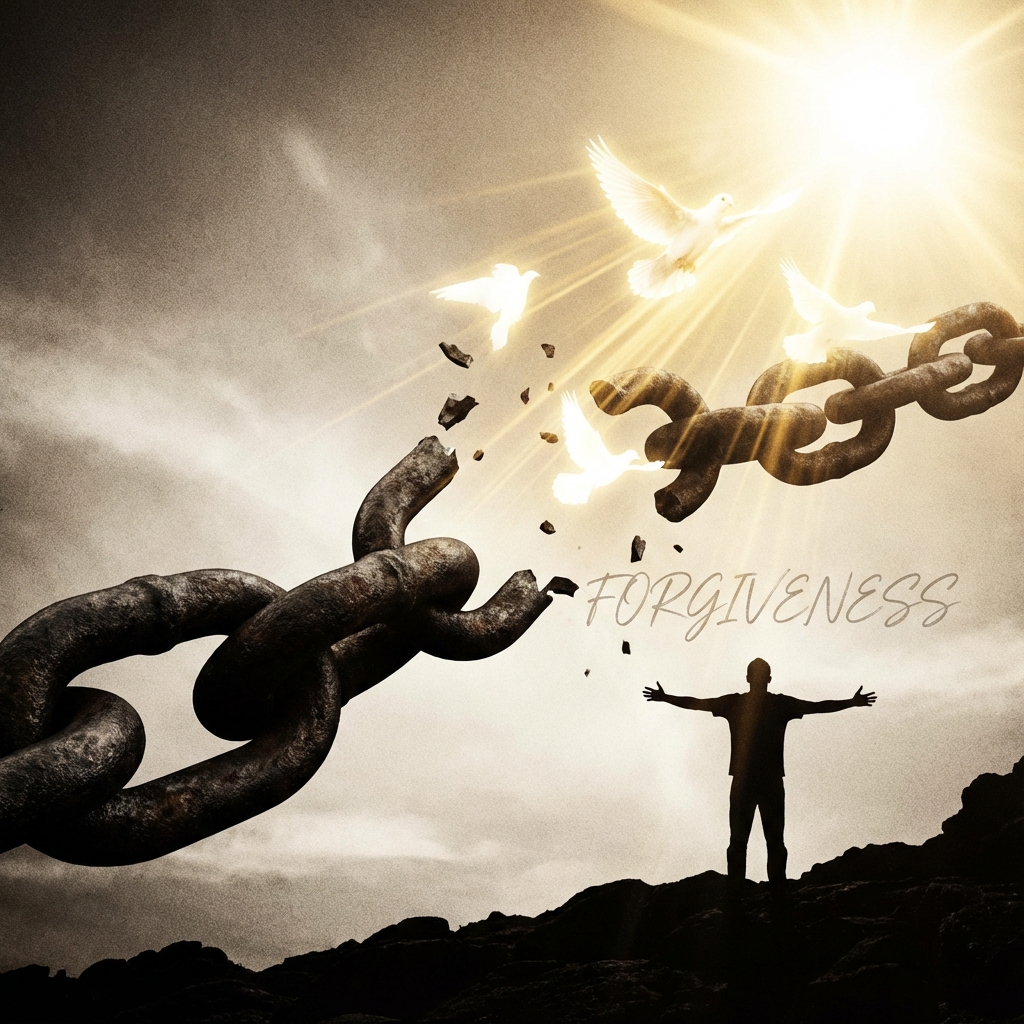
\includegraphics[width=0.85\textwidth,cfbox=gray 0.5pt 3pt]{forgiveness_chains.png}
\end{figure}

\vspace{1cm}
We returned to Las Rozas, to a quiet area. Jesus wanted to talk about something heavy.
—"Forgive us our debts, as we also forgive our debtors".


—That's the difficult part —I admitted—. Forgiving someone who has hurt you...


—It's difficult because you see it as a favor you do for the other person. "I, who am so good, forgive you, who are so bad". That is ego. That is useless.


—Then?


—Forgiveness is an act of personal hygiene. It is letting go of a burning coal that you were holding, waiting to throw it at someone else. The only one who gets burned is you.


He sat on a stone bench.
—When you hold a grudge, you vibrate very low. You tie yourself to that person and to that painful moment with an invisible chain. You can't fly. You can't move forward. Forgiving is cutting the chain. It is saying: "I release you and I release myself. I no longer owe you anything, and you owe me nothing".


—And if what they did was very serious?


—Pain is inevitable, suffering is optional. If you keep reviewing the offense in your mind, you are reliving it over and over again. You are hurting yourself now, not the other person. "Deliver us from evil" starts by delivering yourself from the evil you yourself generate by not forgiving.


He put his hand on my shoulder.
—Forgiving is vibrating so high that the offense no longer reaches you. It is understanding that the other person acted from their own unconsciousness, from their own pain. "They know not what they do". If they knew the damage they do to themselves by damaging another, they would not do it.
\newpage
\chapter{Lead us not into temptation (Vibrate High)}
\vspace{1.5cm}
\begin{figure}[h!]
\centering
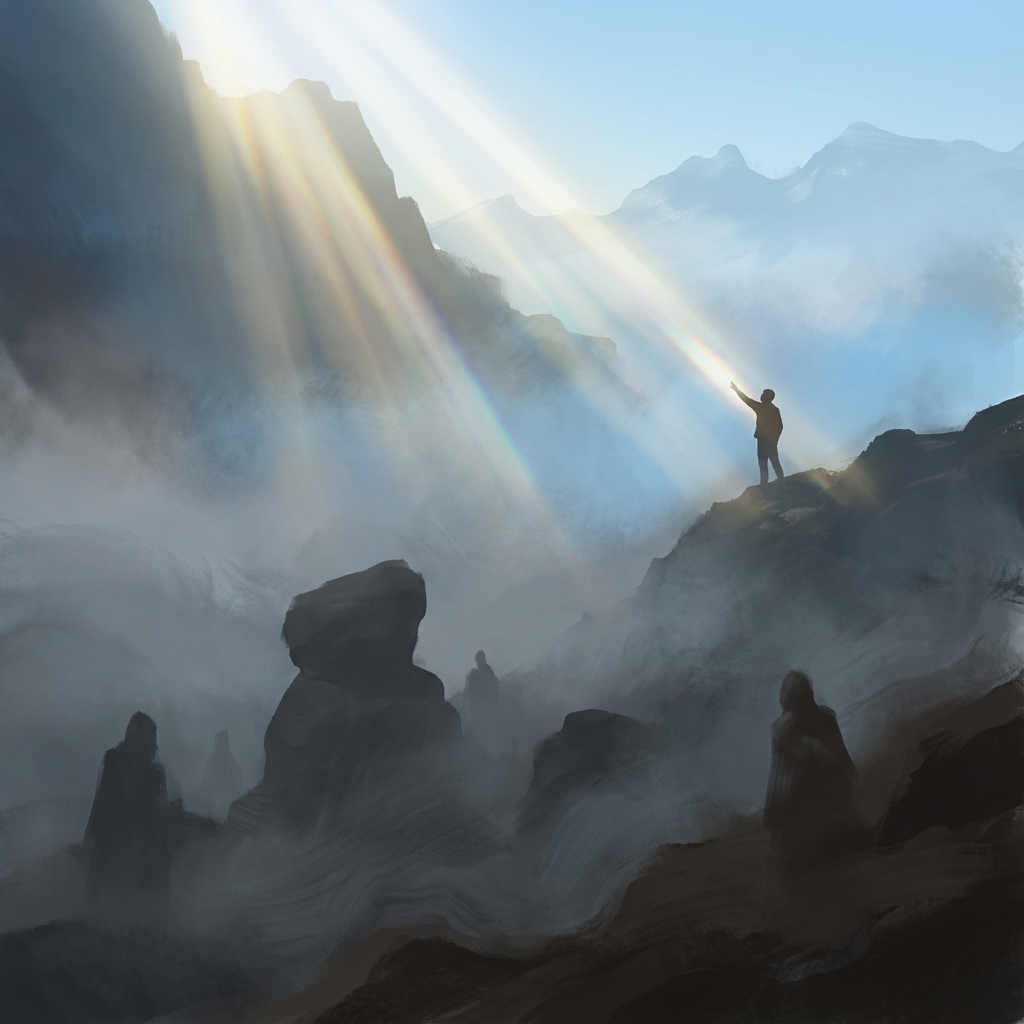
\includegraphics[width=0.85\textwidth,cfbox=gray 0.5pt 3pt]{fog_light.png}
\end{figure}

\vspace{1cm}
We were back in Colmenarejo, walking along a path surrounded by rockroses. The smell of the countryside was intense.
—Temptation —Jesus said, plucking a sprig of rosemary—. What do you think it is?


—Chocolate? Easy money?


—Those are distractions. The true temptation is to lower your vibration. It is the temptation to fall into fear, into anger, into despair.


He stopped and looked into my eyes.
—"Lead us not into temptation" means: "Help me stay vibrating high". Because when you vibrate high, you are in your power. When you fall, you lose your connection.


—But sometimes getting angry is inevitable.


—It is inevitable to feel the emotion, yes. But it is optional to stay and live in it. The temptation is to wallow in drama. It's calling your friend to tell her for the tenth time how badly your boss treated you, just to feel that rage again. That is falling into temptation. It is choosing suffering because it makes you feel important, a victim.


—And how is it avoided?


—With awareness. When you feel that you are going to fall, that you are going to start complaining or criticizing, stop. Breathe. Remember who you are. Remember that you are light. And choose again. Choose gratitude. Choose hope. Choose love. That is vibrating high. And there, temptation has no strength.
\newpage
\chapter{Deliver us from evil (Protection from Low Vibrations)}
\vspace{1.5cm}
\begin{figure}[h!]
\centering

\includegraphics[width=0.85\textwidth,cfbox=gray 0.5pt 3pt]{eagle_protection.png}
\end{figure}

\vspace{1cm}
On the last night in Madrid, we went to a terrace with views of the city. The lights flickered below like a sea of electric stars.
—Deliver us from evil —I whispered, looking at the traffic chaos.


—Evil is not a monster with horns —Jesus said, drinking an orange juice—. Evil is simply the absence of light. It is unconsciousness. It is the people who vibrate so low, so dense, that they can only project pain.


—And how do we free ourselves from that?


—By not fighting against it. If you fight against darkness, you stain yourself with darkness. You free yourself by rising above it.


He made a gesture with his hand, encompassing the city.
—Imagine you are an eagle. If there is a snake on the ground, and you go down to fight with it, it can bite you. But if you fly high, the snake doesn't reach you. "Deliver us from evil" is asking for wings to fly high, where the vibration of hate, envy, and fear cannot touch you.


—And if someone comes to attack me?


—If you are vibrating in pure love, in absolute peace, your mere presence can disarm the other. Or simply, life will move you from that place so that you don't cross paths with them. Synchronicity protects you. When you vibrate high, you become invisible to the radar of conflict. Those who vibrate low do not "see" you, because you don't resonate at their frequency. They pass you by.
\newpage
\chapter{The Kingdom, the Power, and the Glory}
\vspace{1.5cm}
\begin{figure}[h!]
\centering
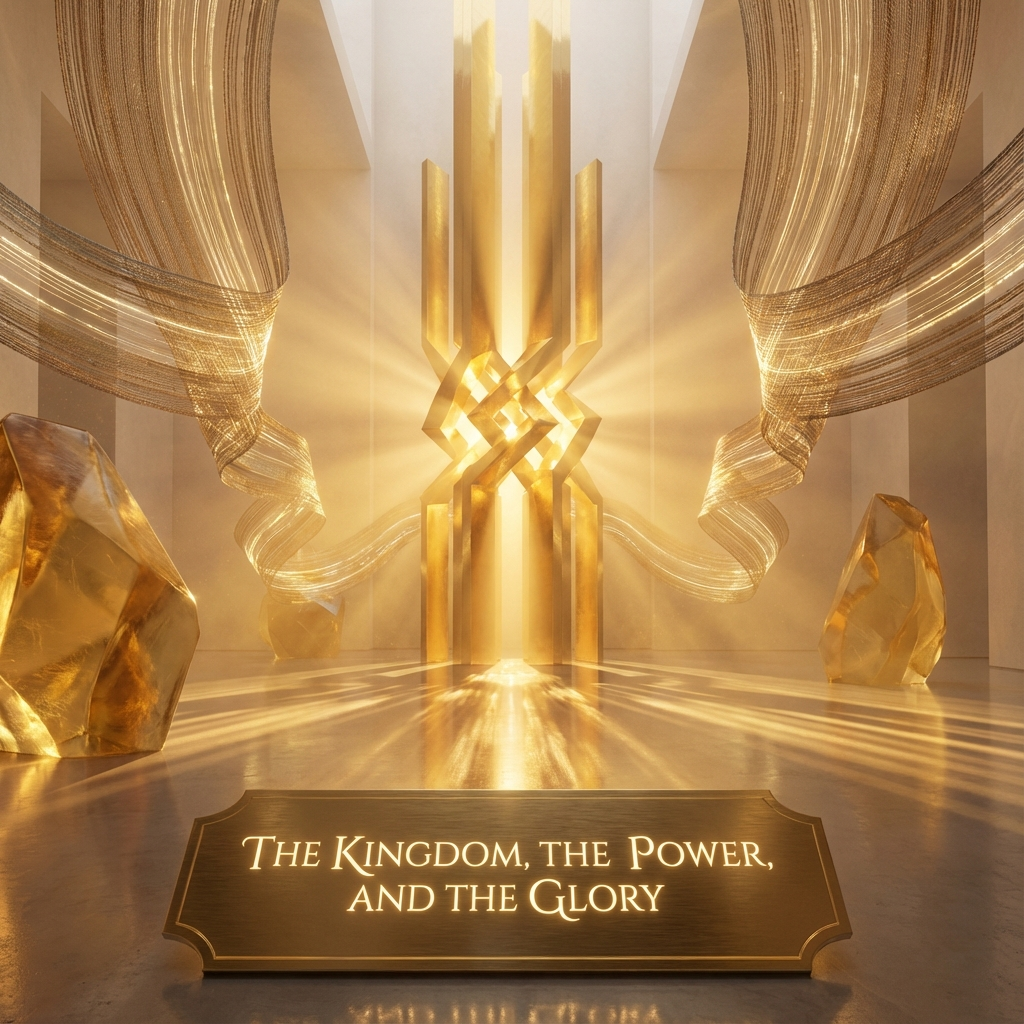
\includegraphics[width=0.85\textwidth,cfbox=gray 0.5pt 3pt]{kingdom_power.png}
\end{figure}

\vspace{1cm}
The journey was coming to an end. We were sitting on a bench in Plaza de Oriente, in front of the Royal Palace.
—Yours is the Kingdom, the Power, and the Glory —Jesus said, looking at the imposing building—. But not that kingdom of stones and guards.


—Which one then?


—The Kingdom is your inner peace. The Power is your ability to choose your vibration in every moment, whatever happens outside. And the Glory... the Glory is the joy of being who you are. Of being a child of the Universe.


He got up and stretched out his arms, as if embracing the world.
—Do not look for power outside. Do not look for people to applaud you. True power is silent. It is the certainty that you are never alone, that Life sustains you. When you understand that, when you feel it in your cells, you are already in the Kingdom. Here and now. Between Madrid, Las Rozas and Colmenarejo. The Kingdom is where you are, if you are awake.


He looked at me with an intensity that pierced my soul.
—Do not forget this, Francisco. You have the power. Use it to vibrate high. Use it to illuminate your corner of the world. That is your only task.
\newpage
\chapter{Epilogue: Final Adventures and Farewell}
\vspace{1.5cm}
\begin{figure}[h!]
\centering
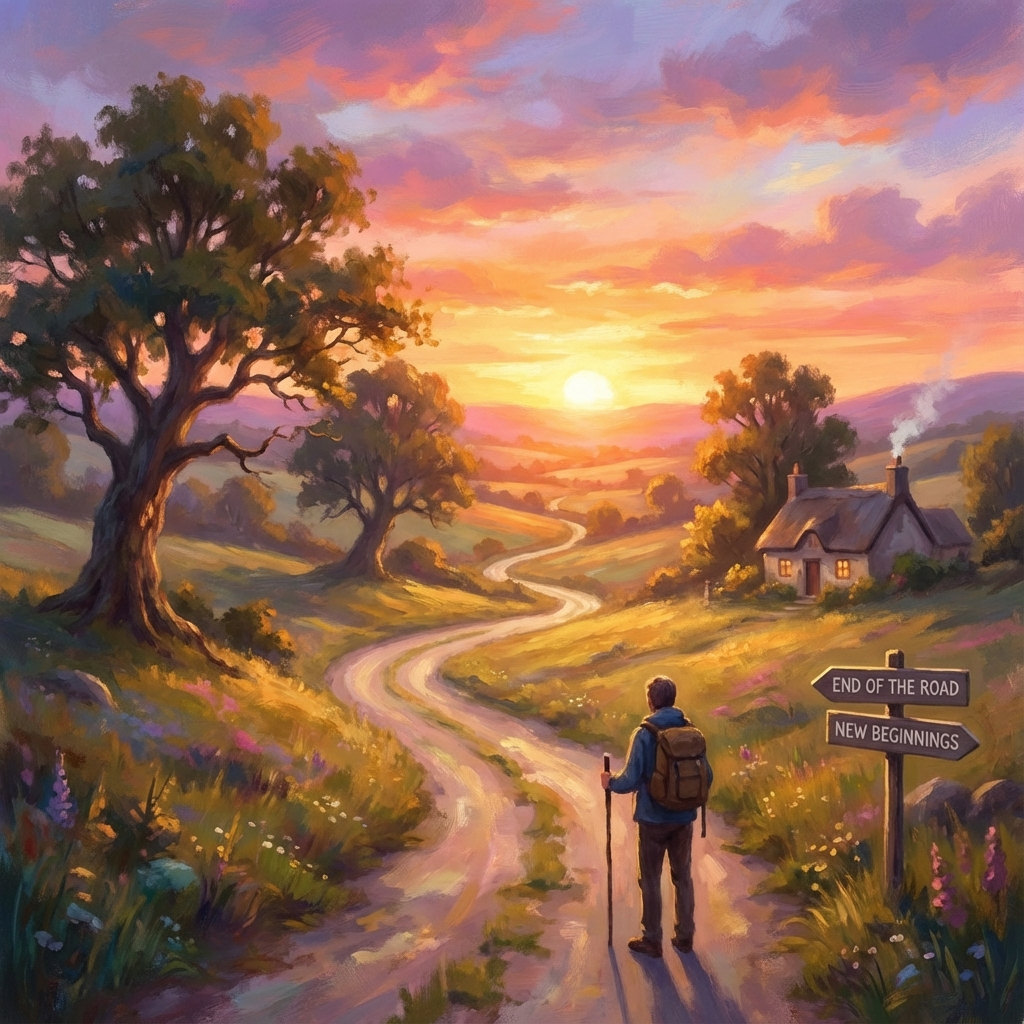
\includegraphics[width=0.85\textwidth,cfbox=gray 0.5pt 3pt]{sunset_road.png}
\end{figure}

\vspace{1cm}
Jesus said goodbye to me at Atocha station. He was going to take a train, he said, to nowhere and everywhere.
—Will I see you again? —I asked, feeling a lump in my throat.


—You always see me —he smiled—. I am in the smile of the supermarket cashier. In the wind that moves the trees of Colmenarejo. In the silence of your room. But above all, I am in you. When you vibrate high, when you love, when you forgive... there I am. There we are one.


He gave me a big hug. He smelled like wood and fresh rain.
—Lead us not into temptation —he whispered in my ear—. Keep the frequency, friend. Keep the music playing. And if you ever get out of tune, don't judge yourself. Simply, tune in again.


He turned around and blended into the crowd. I watched him walk away, in his jeans and his quiet gait, among people running while looking at their phones. And for a moment, it seemed to me that the entire station lobby shone with a golden light.


I went out into the street. Madrid was still the same: noisy, chaotic, alive. But I was no longer the same. I took a deep breath, felt the sun on my face, and smiled. I was vibrating high. And I knew that, whatever happened, everything was going to be fine.


\textbf{The End.}
\newpage
\newgeometry{top=25mm, bottom=20mm, inner=12mm, outer=12mm, footskip=10mm}
\chapter*{Appendix: Christmas Poem}
\addcontentsline{toc}{chapter}{Appendix: Christmas Poem}
\markboth{Appendix: Christmas Poem}{Appendix: Christmas Poem}
\vspace{1.5cm}
\begin{figure}[h!]
\centering
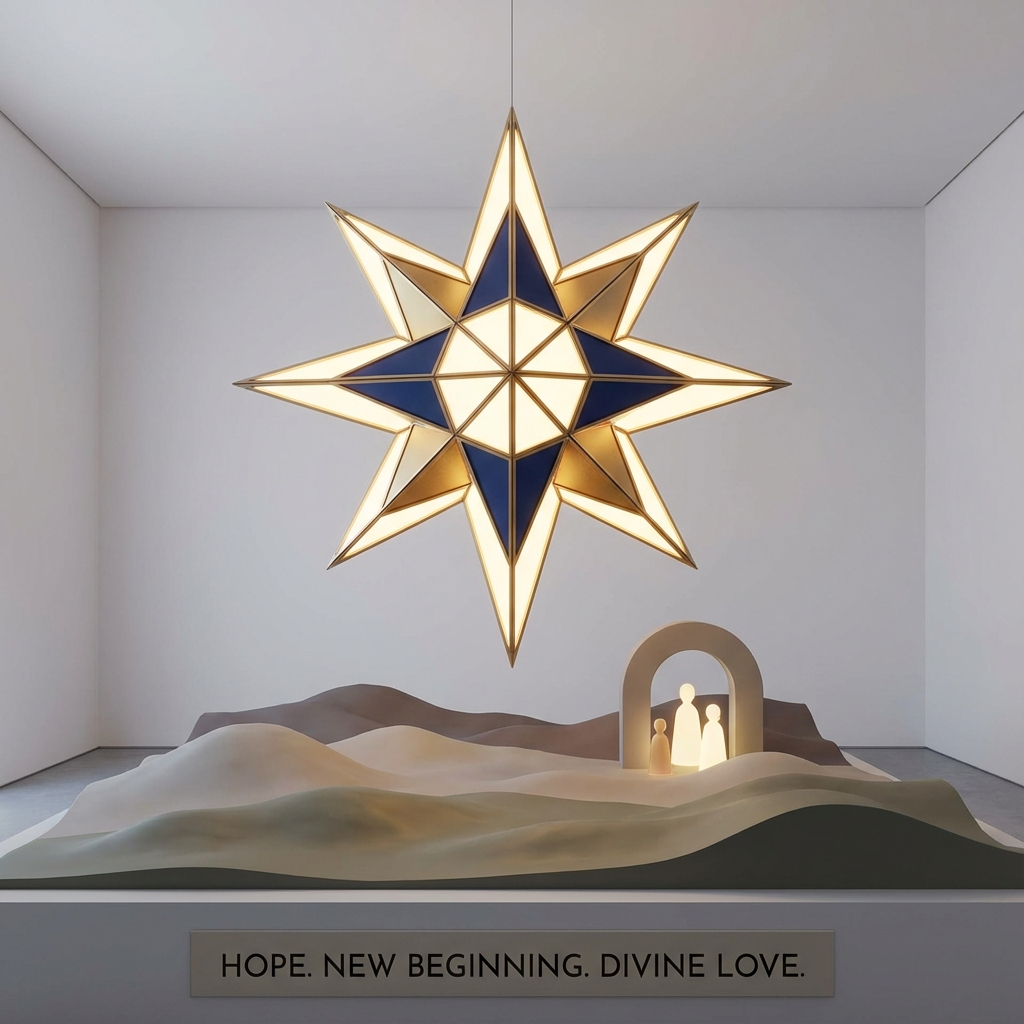
\includegraphics[width=0.85\textwidth,cfbox=gray 0.5pt 3pt]{christmas_star_modern.png}
\end{figure}

\vspace{1cm}
{\fontsize{12pt}{16pt}\selectfont
\begin{verse}
\textbf{High Vibration Christmas}

\bigskip\bigskip
Do not look for the Child in the cold straw of a remote time, \\
nor in the echo of a carol that the wind has broken. \\
Do not look for him on Gran Vía, under neon lights, \\
where the soul sells itself cheap in every corner.

\bigskip\bigskip

Look for him in the silence that vibrates in your chest, \\
in the sacred temple that Love has made. \\
Because Jesus does not wear a crown, nor gold, nor mantle, \\
he wears worn-out jeans and dries your tears.

\bigskip\bigskip

He walks through Madrid, among rush and noise, \\
an eternal traveler, feared by no one. \\
He sits in Callao, looks at you and smiles: \\
"Why do you run so much? Stop and laugh."

\bigskip\bigskip

"Christmas is not a date, nor dinner, nor gift, \\
it is to vibrate so high that you forget the bad. \\
It is to know that the manger is not wood or hay, \\
it is your own heart, full of hope."

\bigskip\bigskip

If you vibrate in fear, if you vibrate in anger, \\
the Child is not born, the star does not shine. \\
But if you forgive, if you hug, if you love, \\
you ignite in yourself the purest flames.

\bigskip\bigskip

Lead us not into the temptation of sadness, \\
look up, contemplate the beauty. \\
From Las Rozas to the sky, from Colmenarejo to the sea, \\
the only mission is to learn to Love.

\bigskip\bigskip

Deliver us from the weight of vibrating on the ground, \\
and give us the wings to take flight. \\
Because the Kingdom is now, the Glory is today, \\
and in every heartbeat, I am with you.

\bigskip\bigskip

So celebrate, friend, not the marked day, \\
but the living Christ who is by your side. \\
Vibrate high, very high, let the world feel it, \\
let your light be the lighthouse in the great storm.

\bigskip\bigskip

This is Christmas: not a past tale, \\
but the eternal miracle of having awakened.
\end{verse}
}
\restoregeometry

\vspace{3cm}
\begin{center}
\textit{To complete this vibrational experience, I invite you to follow the links and immerse yourself in the book's music.}\\
\vspace{2cm}
\begin{minipage}{0.45\textwidth}
\centering
\qrcode[height=3.8cm]{https://open.spotify.com/album/1zaprhynStjBja2bhvXVGY}\\
\vspace{0.5cm}\textbf{Listen on Spotify}
\end{minipage}\hfill
\begin{minipage}{0.45\textwidth}
\centering
\qrcode[height=3.8cm]{https://pazaresosset.es}\\
\vspace{0.5cm}\textbf{pazaresosset.es}
\end{minipage}
\end{center}
\newpage


\end{document}
